This chapter presents the design and implementation of \bpfbox{}, an initial research
prototype of an \gls{ebpf}-based confinement framework. \bpfbox{} is the first
full-fledged confinement framework to leverage \gls{krsi}'s \gls{lsm} programs to enforce
high-level policy. Using \gls{ebpf}, it combines various behavioural aspects of the
sandboxed application from both userspace and kernelspace to enforce a simple, yet
fine-grained policy defined in a domain-specific policy language. This chapter was a part
of a previously published paper at CCSW'2020, co-authored with Anil Somayaji and David
Barrera~\cite{findlay2020_bpfbox}.



\section{\bpfbox{} Overview}

At a high level, \bpfbox{} is a confinement mechanism based on \gls{ebpf}. \todo{Outline basic components}

\todo{Describe how \bpfbox{} enforces policy from start to finish, refer to \Cref{fig:bpfbox-overview}}

\begin{figure}[htpb]
  \centering
  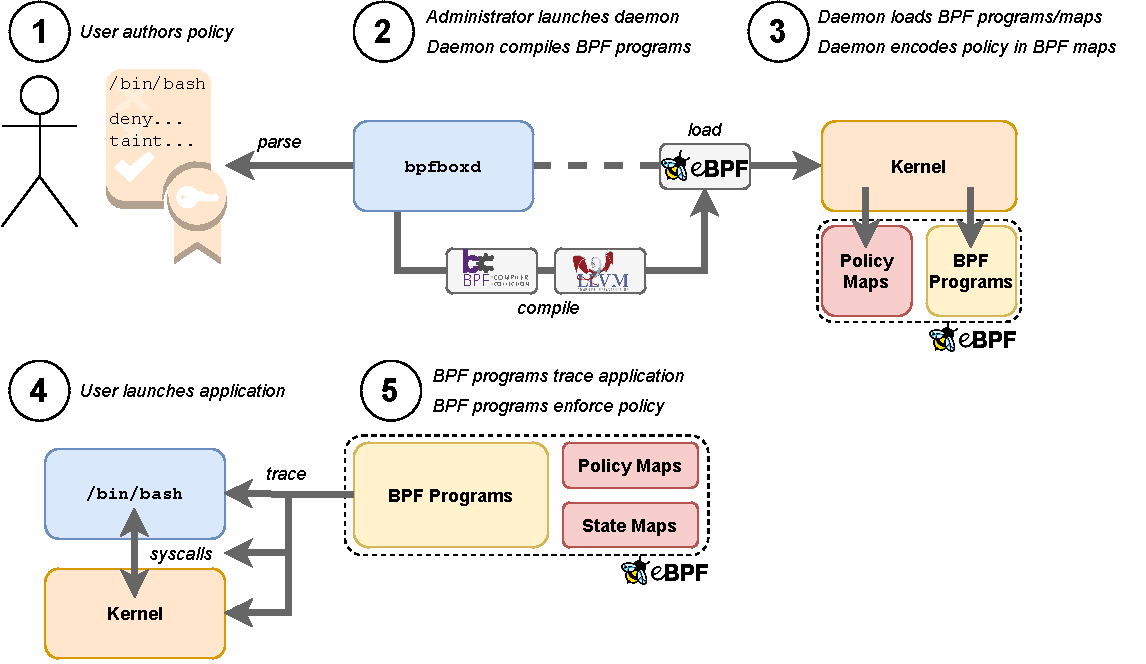
\includegraphics[width=0.8\linewidth]{figs/bpfbox/overview.pdf}
  \caption[A high-level overview of how \bpfbox{} confines applications]{
    A high-level overview of how \bpfbox{} confines applications. Users write policy files
    which the daemon encodes into \gls{ebpf} maps. The daemon loads these maps, along with
    policy enforcement and tracing programs into the kernel. At runtime, \bpfbox{}'s
    \gls{bpf} programs trace the application and enforce policy.
  }%
  \label{fig:bpfbox-overview}
\end{figure}

\bpfbox{}'s fundamental enforcement strategy is based on several \gls{bpf} program and map
types, summarized as follows. The reader is encouraged to revisit
\Cref{ss:bpf-programs-bg,ss:bpf-maps-bg} in \Cref{c:background} for clarification on
specific programs and maps.

\begin{itemize}
  \item \textbf{State Maps} are \gls{ebpf} hash maps that associate a kernel \gls{tgid}
  with a specific task state. The task state holds information including policy
  association, task liveness, and other metadata used for enforcement.

  \item \textbf{Policy Maps} are \gls{ebpf} hash maps that encode \bpfbox{} policy for
  various categories of access. Each map encodes an access vector and policy ID pair that
  is mapped to the corresponding enforcement decision. At runtime, \bpfbox{} queries these
  maps before making an enforcement decision on a specific access pattern.

  \item \textbf{Tracepoints} enable \bpfbox{} to track the state of a process from the
  point where it forks or executes a new binary to when it exits. \bpfbox{} stores
  per-process state from its tracepoints in \textit{state maps} for later use.

  \item \textbf{\gls{lsm} Probes} enforce policy by attaching to \gls{lsm} hooks in the
  kernel. These hooks are called by kernel functions such as system call implementations
  and trigger the corresponding \gls{bpf} program, which enforces a policy decision on the
  target application. To enforce policy, \bpfbox{}'s \gls{lsm} probes query \textit{policy
  maps} and \textit{state maps}.

  \item \textbf{Kprobes and Uprobes} are used to enforce \textit{stateful policy},
  according to what function calls a process has made, in kernelspace and userspace
  respectively. A \bpfbox{} policy file may outline that certain rules should only apply
  within the context of a specific function call; when a process runs some code that
  results in such a function call, the corresponding kprobe or uprobe will make an update
  to the process' \textit{state map} to indicate this. \bpfbox{} then considers this state
  when making later enforcement decisions.
\end{itemize}


\section{\bpfbox{} Implementation}

\todo{This section will present the implementation details of \bpfbox{}, taken from our paper.}




\section{\bpfbox{} Policy Language}

\todo{This section will present and document the policy language of \bpfbox{}, taken from our paper.}





\section{Limitations and the Transition Toward \bpfcontain{}}

\todo{This section will discuss limitations of \bpfbox{}, how it was a rough first-cut at
a solution to the confinement problem, and talk about the aspects of \bpfbox{} that
\bpfcontain{} improves upon.}

\begin{inprogress}
\begin{itemize}
  \item
\end{itemize}
\end{inprogress}
